\section{Role of Smart Phone}

\begin{figure}[t!]
  \centering
    \begin{minipage}{0.25\textwidth}
      \centering
        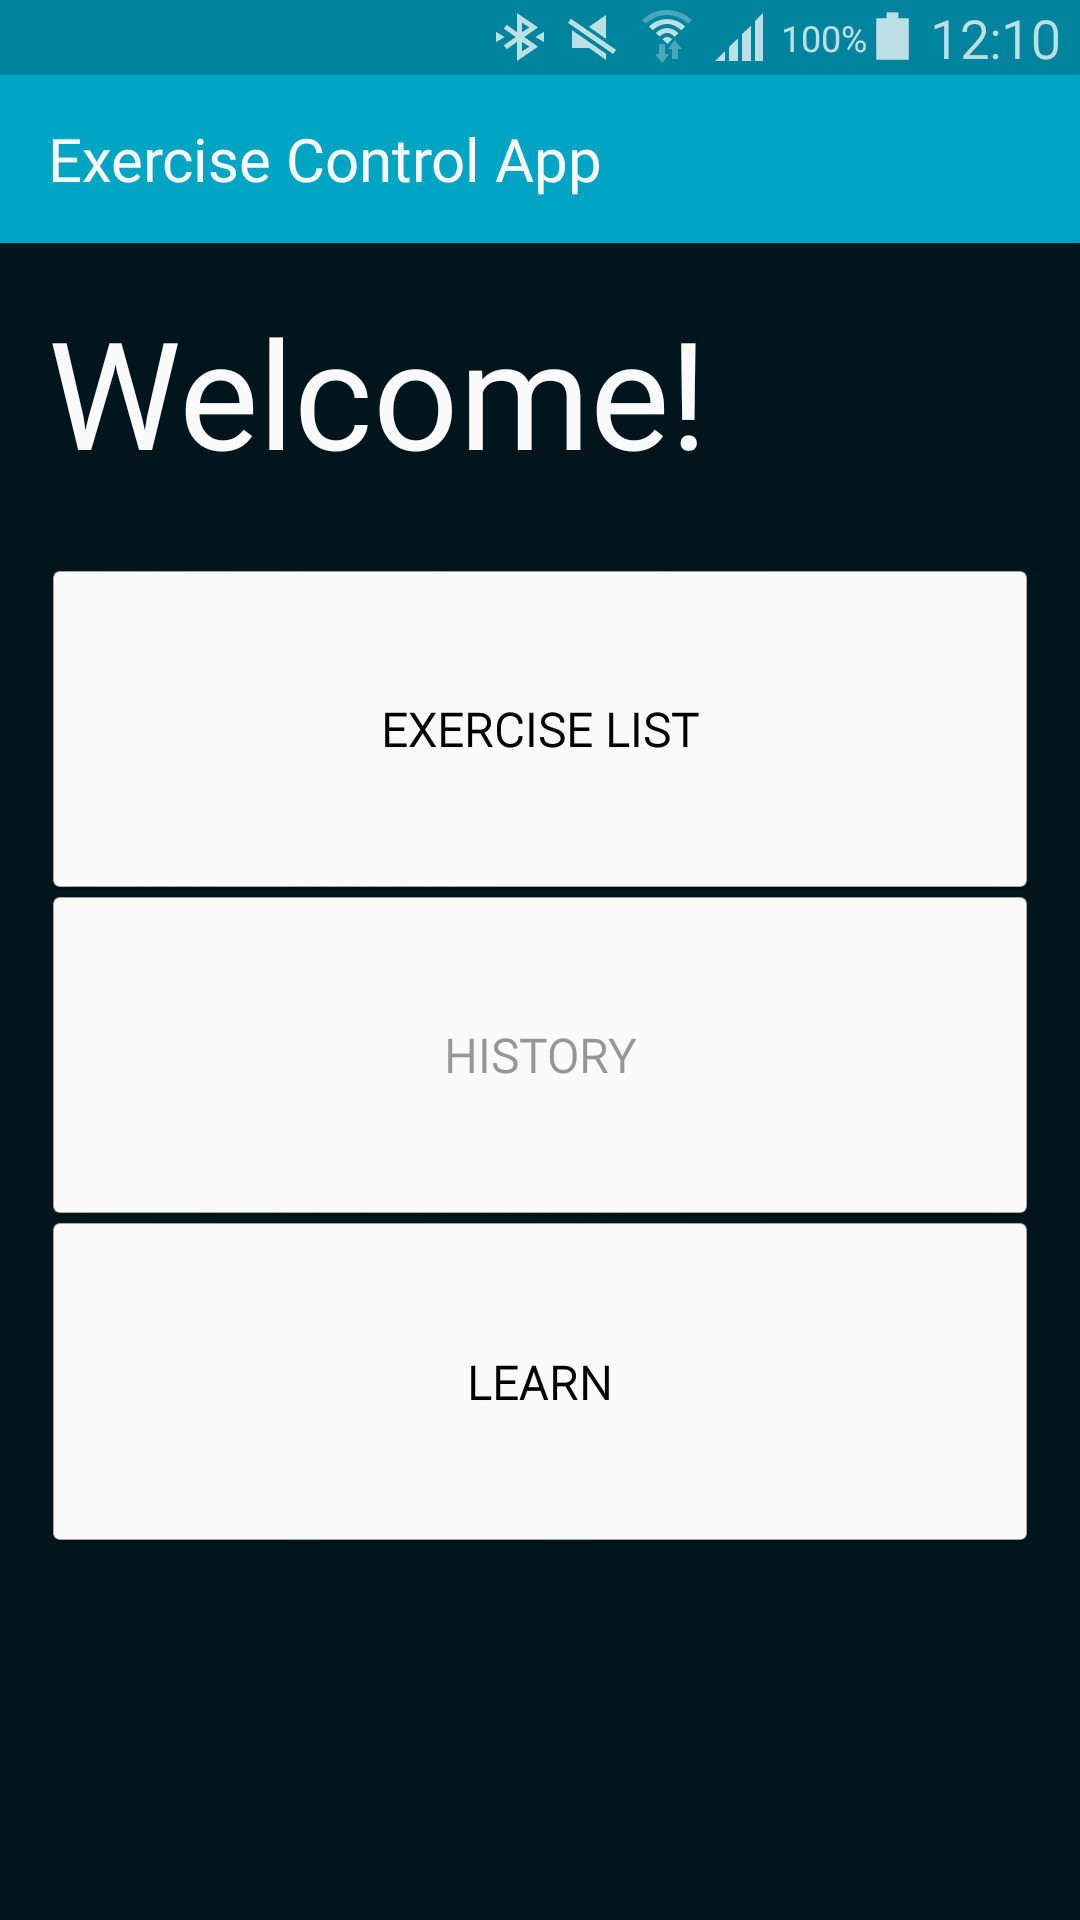
\includegraphics[width=0.80\textwidth]{00_resources/figures/Android_Phone_MainView.png}
    \end{minipage}
    \begin{minipage}{0.25\textwidth}
      \centering
        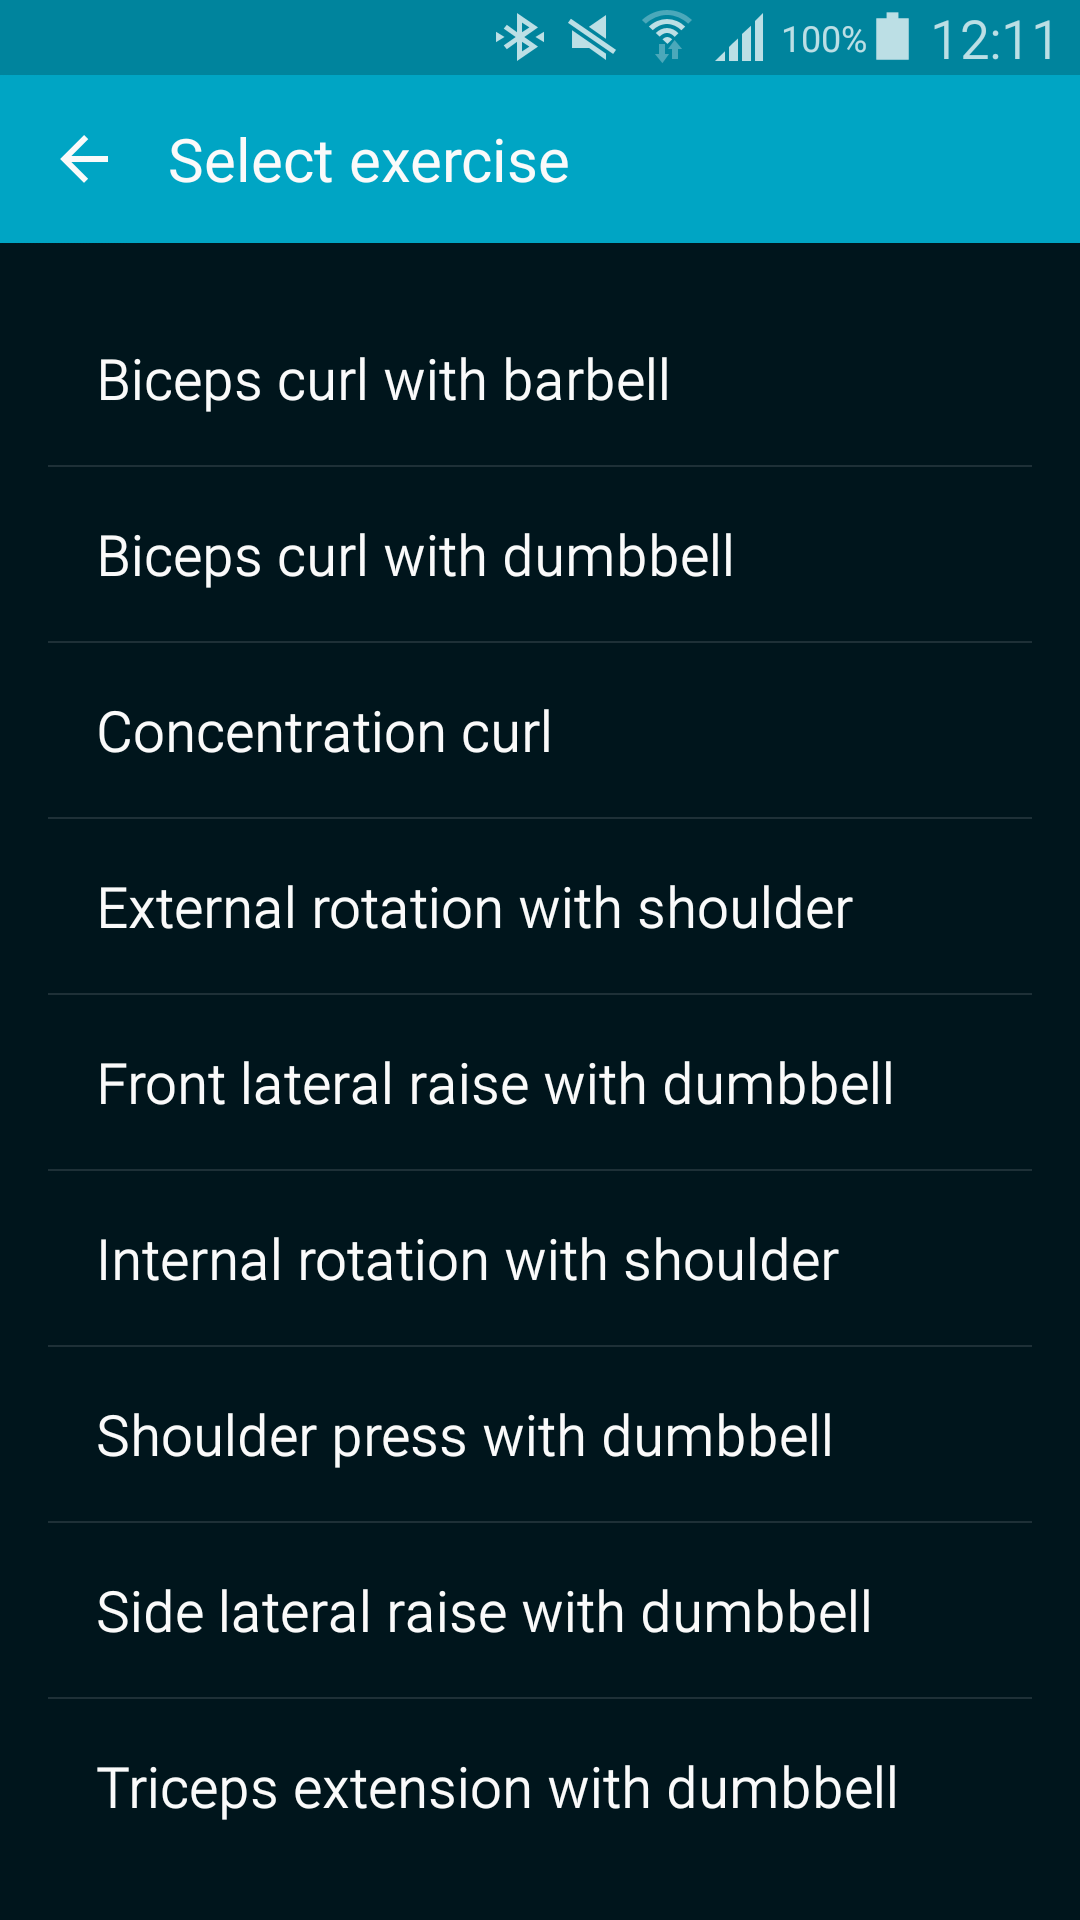
\includegraphics[width=0.80\textwidth]{00_resources/figures/Android_Phone_ListView.png}
    \end{minipage}
    \begin{minipage}{0.25\textwidth}
      \centering
        
\includegraphics[width=0.80\textwidth]{00_resources/figures/Android_Phone_DescriptionView.png}
    \end{minipage}
  \caption{Smart phone user interface}
  \label{fig:smpui}
\end{figure}

The smart phone \textit{Android} application provides a user interface allowing
the user to obtain information about available exercises including a video
demonstration as can be seen in figure \ref{fig:smpui}.

The main purpose, however, is to compare sensory data obtained from the coupled
smart watch against already existing data to determine the degree to which
the exercise has been performed correctly by the user. The computed result is
then shown on the smart watch for user convenience as shown in figure
\ref{fig:smwui}.

Before the application can determine the degree of correctness for a given
exercise, the user has to perform the exercise correctly a number of times to
train the algorithm used within the application. This is preferably done in
the presence of a qualified personal trainer or physiotherapist.
